\cotefile{93}
\scanpage{207}

On a donc

\diagram{\begin{tikzcd}[ampersand replacement=\&,column sep=small,row sep=small]
\llap{(2.1)\qquad}0 \arrow[r] \& P^{ci}_{X/S}\arrow[r] \& P^c_{X/S}\arrow[r,"\text{courbure}"] \& f_*^{\mathrm{fl}}(Z^2_{X/S}) \\
\&\&\& f_*^{\mathrm{fl}}(\Omega^2_{X/S})\arrow[u,phantom,"\rotatebox{-90}{$\subset$}" description]
\end{tikzcd}}

ou, si on préfère, dans le cas où $X$ est lisse sur $S$.

\[
0\longrightarrow\frac{f_*^{\mathrm{fl}}(\underline{Z}^1_{X/S})}{\underline{\mathrm{Im}}\,f_*^{\mathrm{fl}}(\underline O^*_{X/S})}
\longrightarrow P^{ci}_{X/S}\longrightarrow\underline{\mathrm{Pic}}_{X/S}
\longrightarrow R^{2}f_*^{\mathrm{fl}}(0\to\underline\Omega^1_{X/S}\to\underline\Omega^2_{X/S}\to\unsure{\cdots})
\tag*{\unsure{(1.2)|(2.2)}}
\]

[Dans le cas non lisse, on remplace le dernier terme par \deleted{$R^{\unsure{2}}f_*^{\mathrm{cris}}(\unsure{\mathscr J|\mathscr I})$} le faisceau associé à $S'\longmapsto R^2 f_{\underline{S'}\,\mathrm{com}}(\mathscr J_{X_{S'}/S'})$ \inserted{idéal d'augmentation du $(X_{S'}/S')\,\mathrm{cris}$}]

% slanted
\margin{\unsure{pourrait|peut entrer|pour entrer|remis} dans $1^\circ$)}

\uline{Cas particulier} Plaçons nous \unsure{sur|dans} le cas où $\underline{\mathrm{Pic}}^0_{X/S}$ est un schéma abélien $B$, dont le dual est noté $A^0=\underline{\mathrm{Alb}}^0_{X/S}$.

On a alors $X\to\underline{\mathrm{Alb}}^1_{X/S}=A^1$ (torseur sous $A^0$), et supposons que
\diagram{\begin{tikzcd}[ampersand replacement=\&,column sep=tiny,row sep=tiny]
X\arrow[rr,dash]\arrow[dr,dash,"f"'] \& \& A^1\arrow[dl,dash,"\unsure{g^1|g^2}"] \\
\& S \&
\end{tikzcd}}
induise un \uline{isom} $f_*^{\mathrm{fl}}(\Omega^1_{X/S})\longleftarrow {g^1}_*^{\mathrm{fl}}(\Omega^1_{A^1/S})$.

Il suffit pour ceci que \inserted{$f$ pr. plat, que} $\Omega^1_{X/S}$ \deleted{soit} \inserted{plat et} coh.\ plat en dim 0, et que l'on ait isom des $H^0(A^1_s,\Omega^1_{A^1_s/s})\to H^0(X,\Omega^1_{X_s/s})$ fibre à fibre. C'est le cas en particulier si $X$ est un torseur sous schéma abélien (bien sûr), ou si $X$ est une courbe relative propre et lisse.

Alors $P^{c\unsure{0|o}}_{X/S}$ \inserted{de (1.3)} est une extension du schéma abélien $B$ par un fibré vectoriel, et on constate que c'est l'\uline{extension universelle} [compte tenu que $B^*\simeq A$, \deleted{${\unsure{\underline{\mathrm{Lie}}}}_{B^*/\unsure{S}}$} $\underline{\mathrm{Lie}}(B^*)^\vee=\underline{\mathrm{Lie}}(A)^\vee\simeq {g^0}_*(\Omega^1_{\unsure{A^1|A}/S})\simeq {g^1}_*(\Omega^1_{A^1/S})\simeq f_*(\Omega^1_{A^1/S})\ldots$

% archive sheet number: 206
\scanpage{208}

Considérons la suite exacte \unsure{(1.2)|(2.2)}, et $u^*(P^c_{X/S})\to P^c_{X/S}$, je dis qu'en fait

\[
u^*(P^c_{X/S})\longrightarrow P^{ci}_{X/S},\tag*{(2.3)}
\]

\deleted{En effet} dès que l'on a

\[
f_*^{\mathrm{fl}}(\Omega^1_{X/S})=f_*^{\mathrm{fl}}(\underline Z^1_{X/S})\tag*{(2.4)}
\]

\margin{$2$}

(Attention, \deleted{dans la \unsure{définition|différentielles}} \inserted{la notation} de $f_*^{\mathrm{fl}}(\underline Z^1_{X/S})$ \deleted{est faisceau} \inserted{un abus de} $\underline Z^1_{\unsure{X/S|T/S}}$ lang.\ \unsure{pr|les} pour $\mathrm{Ker}\,(f_*^{\mathrm{fl}}(\underline\Omega^1_{X/S})\longrightarrow f_*^{\mathrm{fl}}(\underline\Omega^2_{X/S}))$], et que

\deleted{En effet, en \unsure{lisant} $u^*(P^c)\longrightarrow$}

\[
\deleted{f_*^{\mathrm{fl}}(\unsure{\Omega})} V=f_*(\underline\Omega^2_{X/S})\ \deleted{\unsure{\text{est}}}\ \deleted{\text{est}}\ \text{coreprésentable par un module}\tag*{(2.5)}
\]
quasi-cohérent, \uline{ou} représentable par un fibré vectoriel.

En effet, on a alors $\mathrm{Hom}(B,V\deleted{f_*(\Omega^{\unsure{1}}_{X/S})})=0$, donc $\mathrm{Hom}(u^*(P^c),V)\longrightarrow\mathrm{Hom}(f_*^{\mathrm{fl}}(\Omega^1_{X/S})/{-},V)$ est injectif, \deleted{donc} or l'hom obtenu est la différentielle ext. $f_*^{\mathrm{fl}}(\Omega^1_{\unsure{Y|X}/S})\longrightarrow f_*^{\mathrm{fl}}(\Omega^2_{X/S})$, qui est supposée nulle \ldots.

En particulier, sous les conditions favorables (2.2), et moyennant (2.4) et (2.5), on a

\[
(P^{c\unsure{0|o}})\subset P^{ci}\qquad\text{i.e.}\qquad P^{c0}=P^{ci0}\tag*{(2.6)}
\]

\textcircled{3}. Supposons que $p\cdot1_S=0$ ($p$ un nb premier). On définit alors

\[
P^{cip}_{X/S}\subset P^{ci}_{X/S}
\]

le sous-faisceau correspondant aux modules à connexions \uline{compatibles aux puiss.\ $p^{\mathrm{ièmes}}$} \deleted{à puissances $p^{\mathrm{ièmes}}$ nulles}. Supposons que $X/S$ ait loc. une $p$-base, alors on a

\[
0\longrightarrow P^{cip}_{X/S}\longrightarrow P^{ci}_{X/S}
\xrightarrow[\substack{\text{tenseur de}\\\deleted{\unsure{\text{défaut de}}}\\\text{$p$-courbure}\\=\deleted{\unsure{\text{obstruction}}}\,\text{de comp. aux puiss. $p^{\mathrm{ièmes}}$}}]{\overset{\inserted{\text{$p$-courbure}}}{K}}
 f_*^{\mathrm{fl}}(\Omega^{1\otimes p}_{X/S})\tag*{(3.1)}
\]

% archive sheet number: 207
\scanpage{209}

\uline{Question} Soit $E$ module à connexion \deleted{intégrable}\inserted{à courbure nulle} sur $X/S$ en car. $p>0$. Peut-on définir un tenseur \deleted{\unsure{dit de}} $p$-courbure sur $X$, qui soit

\[
K\in\Gamma(X,\underline{\mathrm{End}}(E)\otimes(\Omega^{\deleted{\unsure{\otimes p}}1}_{X/S})^{\otimes p})\qquad ?
\]

On a aussi une \deleted{\unsure{hom|homomorphie}} suite exacte, où $\underline{\mathrm{Pic}}^{ci}_{X/S}$ désigne l'image de \deleted{$\unsure{\mathrm{Pic}}$} $P^{ci}_{X/S}\longrightarrow\underline{\mathrm{Pic}}_{X/S}$ (cf. (2.2) dans le cas lisse)

\[
0\longrightarrow
\underbrace{[f_*^{\mathrm{fl}}(\underline O^*_{X/S})\longrightarrow \overset{\inserted{\substack{\text{(défaut d'exactitude}\\\text{dans le milieu)}}}}{f_*^{\mathrm{fl}}(\underline Z^1_{X/S})}\longrightarrow f_*^{\mathrm{fl}}(\underline\Omega^{1\otimes p}_{X/S})]}_{\underline{\mathrm{Cart}}_{X/S}\ \text{``faisceau de Cartier''}}
\longrightarrow P^{cip}_{X/S}\longrightarrow\underline{\mathrm{Pic}}^{ci}_{X/S}
\longrightarrow f_*^{\mathrm{fl}}(\Omega^{1\otimes p}_{X/S})/\mathrm{Im}\,f_*^{\mathrm{fl}}(\underline Z^1_{X/S}),
\tag*{(3.2)}
\]

où la flèche

\[
K_0\colon f_*^{\mathrm{fl}}(\underline Z^1_{X/S})\longrightarrow f_*^{\mathrm{fl}}(\underline\Omega^{1\otimes p}_{X/S})
\]
est donnée par

\[
K_0(\omega)=\omega^{\otimes p}-{\unsure{F|f}}_{X/S}^*(\underbrace{\widetilde C}_{\text{\inserted{opération de Cartier}}}\omega)\qquad\text{pour $d\omega=0$,}\tag*{(3.3)}
\]

\uline{NB} $K_0$ \inserted{est additif mais} n'est pas linéaire, c'est la somme d'une opération $p$-linéaire et d'une opération linéaire.

Tjrs dans le cas de l'existence locale d'une $p$-base, on sait qu'\deleted{\unsure{un}}\inserted{pour un} module \deleted{inversible} qu. coh. $E$ sur $X$, la donnée d'une connexion à courbure et $p$-courbure nulles \deleted{\unsure{éq}} sur $E$ équivaut à celle d'une \uline{donnée} \uline{de descente} de $E$ à $\Lambda=\deleted{\underline O_{\unsure{S|X}}^p}\underline O_S[\underline O_X^p]\simeq\underline O_{X^{p/S}}/J$, où $J$ est le noyau de $\underline O_{X^{p/S}}\longrightarrow F_{X/S\,*}(\underline O_X)$,

\deleted{et qu'une telle donnée de des.} \inserted{La catégorie de ces} $E$ équivaut à celle des modules quasi-cohérents sur $(X^{p/S},\Lambda)\simeq(X,\underline O_X^p)$. Soit $(X^{p/S\,!})$ cet espace annelé, on trouve donc que $P^{cip}_{X/S}$ est le faisceau associé au préfaisceau

\[
S'\longmapsto\mathrm{Pic}(X_{S'}^{p/S'\,!}).
\]

% archive sheet number: 208
\scanpage{210}

Si en particulier pour tt $S'$, $X_{S'}^{p/S'}\deleted{\unsure{\not\sim|\not\ni}}\xleftarrow{\sim} X_{S'}^{p/S'\,!}$, ce qui est le cas en particulier si $X/S$ est \uline{lisse}, on trouve un isom

\[
P^{cip}_{X/S}\simeq \underline{\mathrm{Pic}}^{\deleted{\unsure{cp}}}_{X^{p/S}/S}\simeq\underline{\mathrm{Pic}}_{X/S}^{(p/S)}\tag*{(3.4)}
\]

L'homomorphisme canonique $P^{cip}_{X/S}\to\underline{\mathrm{Pic}}_{X/S}$ n'est alors autre que la Verschiebung

\[
V\colon\underline{\mathrm{Pic}}_{X/S}^{p/S}\longrightarrow\underline{\mathrm{Pic}}_{X/S}\tag*{(3.5)}
\]

[\unsure{encore|avouer|ainsi} qu'il faudrait définir $V$ avec une généralité suffisante pour que ce qu'on vient de dire ait tjrs un sens \ldots]. On trouve donc, en \unsure{vertu} \deleted{\unsure{en}} (3.2), un isom.

\[
\mathrm{Ker}(V_{\underline{\mathrm{Pic}}_{X/S}})\simeq
\left\{\begin{aligned}
&\text{faisceau des \deleted{formes}\inserted{sections} $\omega$ de $f_*^{\mathrm{fl}}(\Omega^1_{X/S})$ telles}\\
&\text{que $d\omega=0$, $\widetilde C\omega=\widetilde\omega$, modulo le sous-}\\
&\text{faisceau des $df/f$, $f$ ds $f_*^{\mathrm{fl}}(\underline O^*_{X/S})$}
\end{aligned}\right.\tag*{\unsure{(3.6)|(2.6)}}
\]

Quand on inverse sur $(\mathrm{Sch})/S$ les \deleted{\unsure{immersions}} morphismes entiers surjectifs radiciels, \inserted{[en fait, il suffit \unsure{pour} certains très particuliers]}, de \deleted{\unsure{sorte}} que $\underline{\mathrm{Pic}}_{X/S}\xrightarrow F\underline{\mathrm{Pic}}_{X/S}^{p/S}$ devient inversible, on trouve que le \deleted{\unsure{deuxième}} premier mbr devient $\,{}_p\underline{\mathrm{Pic}}_{X/S}$ \ldots.

\uline{Comparaison} \deleted{des} $P^{cip\,\unsure{0|o}}_{X/S}$ \uline{et} $P^{cip\,0}_{\mathrm{Alb}^0_{X/S}}$ Plaçons nous pour simplifier dans le cas $X/S$ lisse, de sorte que (3.4) est valable, et supposons que $\underline{\mathrm{Pic}}^0_{X/S}$ soit un schéma abélien $B$. Comme on aura $(\underline{\mathrm{Pic}}^{\deleted{\unsure{p/S}}}_{X/S})^{(p/S)\,0}=(\underline{\mathrm{Pic}}^0_{X/S})^{p/S}=B^{(p/S)}$, \deleted{$\simeq\underline{\mathrm{Pic}}^0_{\unsure{X}}$} \deleted{\unsure{on trouve}} et qu'on a aussi $B\simeq\underline{\mathrm{Pic}}^0_{A^1/S}=\underline{\mathrm{Pic}}^0_{A/S}$,

% archive sheet number: 209
\scanpage{211}

on trouve que

\[
P^{cip\,\unsure{0|o}}_{X/S}\xleftarrow{\sim}P^{cip\,0}_{A^1/S}\simeq P^{cip\,0}_{A^0/S}\simeq B^{(p/S)}\tag*{(3.7)}
\]

i.e. on trouve la m\textsuperscript{e} chose que \unsure{sur|dans} le cas d'un schéma abélien. \inserted{\uline{Remarque}} D'ailleurs, faisant \deleted{\unsure{le}} maintnt $X=A$, on sait que $B^{\unsure{(p/S)|cp0}}$, regardé comme extension de $B$ par un grpe \deleted{$\mathrm{Ker}\ V$}

\[
\alpha_B=\mathrm{Ker}(V_B:B^{p/S}\to B),
\]

qui est un groupe affine sur $S$ annulé par $V$, est l'extension \uline{universelle} de cette nature [du moins \deleted{\unsure{sur un}} si $S$ est le spectre d'un corps parfait].

$D(\alpha_B)=\mathrm{Ker}\,F_{B^*}$ \inserted{\deleted{\unsure{donc}} $F_A$} est un groupe infinitésimal de hauteur 1, dont l'algèbre de Lie est $\underline{\mathrm{Lie}}(B^*)$, et on sait que $\underline{\mathrm{Lie}}(B^*)^\vee$ est l'\uline{enveloppe vectorielle} de ce groupe fini; donc on voit que l'extension vectorielle universelle est déduite par $\alpha_B\longrightarrow\text{enveloppe vectorielle}\simeq\underline{\mathrm{Lie}}(B^*)^\vee$, de l'extension universelle par des groupes annulés par $V$.

4. Supposons que $p$ soit nilpotent sur $S$, sans plus. Soit $P^{cin}\subset P^{ci}$, défini par les connexions à courbure \deleted{nulle}\uline{nilpotentes}. Si $X/S$ est lisse, \deleted{et $S$ réduit, alors il s'agit de connexions} \inserted{les valeurs des foncteurs préc.\ sur les $S'$ \uline{réduits}} sont les \deleted{\unsure{mêmes}} que \deleted{\unsure{les}} ceux de $P^{cip}$; \deleted{et pour $S'$} quelcon-

% archive sheet number: 210
\scanpage{212}

\deleted{pour simplifier, $S$ \inserted{loc.} noeth, donc les $S'$ \deleted{\unsure{tous}} aussi (NB ils sont l. de p.f. sur $S$) \unsure{du lieu|du leur|du livre|dans l'énoncé} \unsure{nilradical|nilradicaux|nilpotents} de \unsure{ce quotient|ce qui précède|(sur $S$)}, on trouve}

On voit que, une connexion à courbure nulle sur un Mod. inversible sur $X_{S'}/S'$ est à courbure \uline{nilpotente} ssi, en restreignant sur $S'_{\mathrm{réd}}$, on trouve connexion compatible aux puissances $p^{\text{ièmes}}$. Donc on trouve que $P^{cin}_{X/S}$ est l'image inverse dans $P^{ci}_{X/S}$ du sous faisceau $\overline{f_*^{\mathrm{fl}}(\Omega^{1\otimes p}_{X/S})}\subset f_*^{\mathrm{fl}}(\Omega^{1\otimes p}_{\unsure{X|x}/S})$, qui est le \deleted{\unsure{sous}} ``grpe $\pm$ formel associé'' \ldots. On trouve ainsi

\[
0\longrightarrow P^{cip}\longrightarrow P^{ci}_{X/S}\longrightarrow f_*^{\mathrm{fl}}(\Omega^{1\otimes p}_{X/S})/\overline{f_*^{\mathrm{fl}}(\Omega^{1\otimes p}_{X/S})}.\tag*{(4.1)}
\]

\deleted{\unsure{4}} et (3.1) devient

\diagram{\begin{tikzcd}[ampersand replacement=\&,column sep=small,row sep=tiny]
\llap{(4.2)\qquad}0\arrow[r]\&P^{cip}_{X/S}\arrow[r]\&P^{cin}_{X/S}\arrow[r]\&\overline{f_*^{\mathrm{fl}}(\Omega^{1\otimes p}_{X/S})},\\
\& \underline{\mathrm{Pic}}_{X/S}^{p/S}\arrow[u,phantom,"\rotatebox{90}{$\simeq$}" description]
\end{tikzcd}}

qui explicite $P^{cin}$ comme extension d'un ss-grpe d'un grpe $\pm$formel par \deleted{\unsure{un}} le grpe $P^{cip}$, qui est bien compris \ldots

\deleted{On peut aussi se proposer d'étudier}

On conclut

\diagram{\begin{tikzcd}[ampersand replacement=\&,column sep=small,row sep=tiny]
\llap{(4.3)\qquad}0\arrow[r]\&P^{cip\,\unsure{0|o}}_{X/S}\arrow[r,dash]\&P^{cin\,0}_{X/S}\arrow[r]\&\overline{f_*^{\mathrm{fl}}(\Omega^{1\otimes p}_{X/S})}.\\
\&\underline{\mathrm{Pic}}_{X/S}^{0\,p/S}\arrow[u,phantom,"\rotatebox{90}{$\simeq$}" description]
\end{tikzcd}}

\deleted{On peut aussi aller en sens inverse, et}

étudier le noyau $U$ \deleted{\unsure{de}} \inserted{\unsure{dans|de}} $P^{cin}_{X/S}\to\underline{\mathrm{Pic}}_{X/S}$,

\[
0\longrightarrow U\longrightarrow P^{cin}_{X/S}\longrightarrow\underline{\mathrm{Pic}}_{X/S}\tag*{(4.4)}
\]

c'est le noyau de $\dfrac{f_*^{\mathrm{fl}}(\underline Z^1_{X/S})}{\mathrm{Im}\,f_*^{\mathrm{fl}}(O^*_{X})}\longrightarrow f_*^{\mathrm{fl}}(\Omega^{1\otimes p}_{X/S})/\overline{f_*^{\mathrm{fl}}(\Omega^{1\otimes p}_{X/S})}$, donc il admet une dévissage en

\[
0\longrightarrow\underline{\mathrm{Cart}}_{X/S}\longrightarrow U\longrightarrow\overline{f_*^{\mathrm{fl}}(\Omega^{1\otimes p}_{X/S})}\tag*{(4.5)}
\]

% archive sheet number: 211
\scanpage{213}

où $\underline{\mathrm{Cart}}_{X\unsure{,|/}S}$ est le faisceau de Cartier déjà envisagé dans (3.2). Regardons le sous foncteur de \deleted{$\unsure{\mathrm{Pic}}$} $P^{cin}_{X/S}$ image inverse de $\underline{\mathrm{Pic}}^0_{X/S}$ et supposons que $\underline{\mathrm{Pic}}^0_{X/S}$ est $V$-divisible (p.ex. un schéma abélien), de sorte que $(\underline{\mathrm{Pic}}^{0\deleted{\unsure{p/S}}}_{X/S})^{p/S}\unsure{\longleftarrow|\longrightarrow|\text{—}}\underline{\mathrm{Pic}}^0_{X/S}$ est un épimorphisme. On trouve donc une suite exacte

\[
0\longrightarrow U\longrightarrow [P^{cin}_{X/S}]^{0\ \substack{\text{(image inverse}\\\text{de }\underline{\mathrm{Pic}}^0_{X/S})}}\longrightarrow\underline{\mathrm{Pic}}^0_{X/S}\longrightarrow0\tag*{(4.6)}
\]

\uline{NB} Une façon commode d'exprimer $P^{cin}_{X/S}$ est de dire que c'est le complété formel de $P^{cip}_{X/S}\simeq\underline{\mathrm{Pic}}_{X/S}^{\deleted{\unsure{p}}(p/S)}\subset P^{ci}$ dans $P^{ci}$. Dans le cas favorable où $P^{ci\,\unsure{0|o}}$ est l'extension vectorielle universelle \inserted{$E$} d'un schéma abélien $\unsure{B|\mathscr B}$ par un grpe vectoriel $V$, on trouve \unsure{par|pour|que} \deleted{$P^{cin\,0}$} donc $B^{p/S}\subset E$, et on \deleted{trouve} \inserted{pour $P^{cin\,0}_{X/S}$} le complété formel \inserted{le long} \unsure{dudit|du dit|déduit|induit} $B^{p/S}$. Sa connaissance est donc nettement plus précise que celle du complété formel \inserted{$\overline E$} de $E$ le long de sa section unité, i.e. le groupe formel associé à $E$.

% archive sheet number: 212
\scanpage{214}

$c^1(L)$ \uline{style \unsure{connexifiant|connexifiante|connexion plate|connexions} et opération de Cartier}

\unsure{$1$|$'$}

% archive sheet number: 213
\scanpage{215}

$X/S$ lisse, on considère $H^*_{\mathrm{DR}}(X/S)={\unsure{\mathbb H|H}}^*(X,\Omega^*_{X\unsure{/|\,}S})$ et $\mathbb H^*(X,{}^1\Omega_{X/S})$, où ${}^1\Omega_{X/S}=[0\to\underset{\text{degré 1}}{\Omega^1_{X/S}}\to\Omega^{\unsure{2}}_{X/S}\to{-}]$

On a suites spectrales aboutissant à l'une et l'autre, et hom de suites spectrales, donnant un hom de suites exactes en bas degrés

\figure{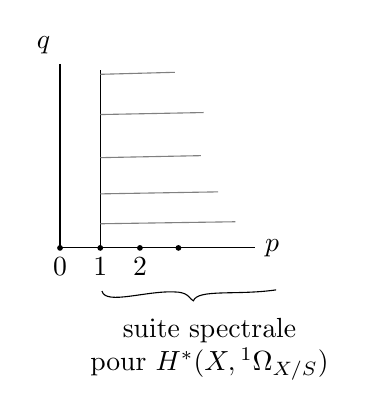
\begin{tikzpicture}[scale=.73]
\draw (0,3.2) node[above left] {$q$} -- (0,0) -- (3.4,0) node[right] {$p$};
\draw (.7,0) -- (.7,3.1);
\foreach \y/\e in {.42/3.05,.94/2.75,1.57/2.45,2.32/2.5,3.02/2.0}{\draw[gray,thin] (.7,\y)--(\e,{\y+.035});}
\foreach \x in {0,.7,1.39,2.06}{\fill (\x,0) circle (.05);}
\node[below] at (0,0){$0$};\node[below] at (.7,0){$1$};\node[below] at (1.39,0){$2$};
\draw (.73,-.75) .. controls (.79,-1.01) and (1.55,-.72) .. (2.06,-.77) .. controls (2.25,-.79) and (2.27,-.91) .. (2.32,-.92) .. controls (2.4,-.71) and (3.07,-.83) .. (3.76,-.73);
\node[below,align=center] at (2.6,-1.05){suite spectrale\\pour $H^*(X,{}^1\Omega_{X/S})$};
\end{tikzpicture}}

\diagram{\resizebox{\linewidth}{!}{\begin{tikzcd}[ampersand replacement=\&,column sep=small,row sep=small]
\&\&{}^{\unsure{1|\prime}}E_2^{10}=Z^1(X,\Omega^*_{X/S})\arrow[ddl]\arrow[d,phantom,"\rotatebox{90}{$\simeq$}" description]
\&\&\&c(\underline L)\arrow[d,phantom,"\rotatebox{-90}{$\in$}" description]
\&\mathrm{Ker}(\mathbb H^1(X,\Omega^1_{X/S})\to H^1(X,\Omega^2_{X/S}))\arrow[d,phantom,"\rotatebox{90}{$\simeq$}" description]\&\\
\&\&H^1(X,{}^1\Omega^*_{X/S})\arrow[d]
\&0\arrow[r]\&{}^1E^{20}_2\arrow[d,phantom,"\rotatebox{90}{$\simeq$}" description]\arrow[r]
\&\mathbb H^2(X,{}^1\Omega^*_{X/S})\arrow[r]\arrow[d]
\&{}^1E_2^{11}\arrow[r]\arrow[d,"\text{surj}"]
\&{}^1E_2^{30}\arrow[d,phantom,"\rotatebox{90}{$\simeq$}" description]\\
0\arrow[r]\&H^1(H^0(X,\Omega^*_{X/S}))\arrow[r]\arrow[d,phantom,"\rotatebox{90}{$=$}" description]
\&H^1_{\mathrm{DR}}(X/S)\arrow[r]
\&\underbrace{\mathrm{Ker}[H^1(X,\underline O_X)\xrightarrow{d}H^1(X,\Omega^1_X)]}_{E^{01}_2}\arrow[r]
\&H^2(H^0(X,\Omega^*))\arrow[r]\arrow[d,phantom,"\rotatebox{90}{$=$}" description]
\&H^2_{\mathrm{DR}}(X)\arrow[r,"\unsure{t}"]
\&H^1(H^1(X,\Omega^*))\arrow[r]\arrow[d,phantom,"\rotatebox{90}{$=$}" description]
\&E_2^{30}\arrow[d,phantom,"\rotatebox{90}{$=$}" description]\\
\&E^{10}_2=\dfrac{Z^1(X,\Omega^*_{X/S})}{\mathrm{Im}\,C^0(X,\Omega^*_{X/S})}
\&\&\&E^{20}_2=\dfrac{Z^2(X,\Omega^*_{X/S})}{\mathrm{Im}\,C^{\unsure{1|0}}(X,\Omega^*_{X/S})}
\&\&E^{11}_2=\dfrac{\mathrm{Ker}[H^1(X,\Omega^1)\to H^1(X,\Omega^2)]}{\mathrm{Im}[H^1(X,\Omega^0)\to H^1(X,\Omega^1]}\&\cdots
\end{tikzcd}}}

Pour que $\exists$ connexion intégrable sur $\underline L$, module inv. donné sur $X$, il faut que l'obstruction en $\mathbb H^2(X,{}^1\Omega^*_{X/S})$ soit nulle, i.e

\textcircled{a} \deleted{$\unsure{H}$} $c^1_{\mathrm{Hdg}}(L)\in H^1(X,\Omega^1_{X/S})$ nul

\textcircled{b} deuxième obstruction dans $H^2(H^0(X,\Omega^*))=\dfrac{Z^2(X,\Omega^*_{X/S})}{\mathrm{Im}\,\unsure{C^1|d}(X,\Omega^{\unsure{0|*}}_{X/S})}$ soit nulle.

\uline{NB} En car. $p>0$, l'obstruction est ds un $\unsure{\mathbb F_p|F_p}$-vectoriel, donc tué par $p$. Donc \inserted{pour} tout élt de $p\,\mathrm{Pic}(X)$ l'obstruction est nulle. On présume, si $X$ est propre sur $S$, \inserted{loclt}, que l'obstruction est nulle \deleted{dans} si $\xi$ est ds $\mathrm{Pic}^0(X/S)$ (à vérifier \ldots).

Supposons l'obstruction en question nulle, \inserted{$S$ de car $p>0$,} Alors l'indétermination pour trouver la connexion intégrable est un $Z^1(X,\Omega^*_{X/S})$, i.e. c'est une 1-forme relative $\omega$ \uline{fermée} ($d\omega=0$). \deleted{A quelle} \deleted{Donc $C$} D'autre part, le \uline{défaut} \uline{de compatibilité} \uline{aux puiss. $p^{\mathrm{ièmes}}$} est un \deleted{homomorphisme} à hom additif et $p$-homogène ${\unsure{\mathscr T|\mathscr U|\underline V}}_{X/S}\longrightarrow\underline{\mathrm{End}}(\underline L)\deleted{\unsure{\simeq}}$, i.e. un hom $u:\mathscr T^{(p)}_{X/S}\longrightarrow\mathrm{End}(\underline L)$, i.e. ici une section de $\underline\Omega^1_{X/S}{}^{(p)}$. Cette section, si on remplace la connexion $\Theta^{{}}$ par $\Theta'=\Theta+\omega$, est remplacée par

% slanted
\margin{résulte des formules explicites}

\[
\begin{aligned}
&\deleted{\xi\longmapsto}u'(\xi)=u(\xi)+\underbrace{\omega(\xi)^p\deleted{\unsure{\omega(\xi)}}+\Theta_\xi^{p-1}\omega(\xi)-\omega(\xi^p)}
=u(\xi)+\underbrace{\omega(\xi)^p-\deleted{\unsure{C_\xi}}\langle\underset{\text{opération de Cartier}}{C}\omega,\widetilde\xi\rangle1_{\unsure{\underline\Lambda|\underline L}}}\\
&=
\end{aligned}
\]

% archive sheet number: 214
\scanpage{216}

% Three long cancellation strokes cross the draft. The oblique marginal note is outside them.
\deleted{La catégorie des objets \unsure{de la forme|de ce genre}}

\diagram{\begin{tikzcd}[ampersand replacement=\&,row sep=small]
\deleted{S}\&\deleted{U_0}\arrow[l,"\deleted{\unsure{\psi_0|\varphi_0}}"']\arrow[d,"\deleted{j}"]\\
\&\deleted{U}
\end{tikzcd}}

\deleted{avec disons $j$ un monomorphisme, \inserted{($S$ fixé)} admet des produits\inserted{ de deux objets} : \deleted{\unsure{pour}} le produit de $(U_0,U)$ et $(V_0,V)$ est $(U_0\times_S V_0,U\times V)$.}

% slanted
\margin{Attention, il n'y a pas d'objet final. par contre il y a des produits fibrés, qui se forment ``terme à terme'', donc des noyaux \ldots}

\deleted{D'autre part le foncteur qui, à $(U,U_0)$ associe le faisceau correspondant sur $D_S$ (ou sur l'un des sous-sites \deleted{$C_S$} \unsure{$A_S$|$C_S$} tel $C_S$ \ldots) commute aux produits (plus gén aux $\varprojlim$ finies \deleted{\unsure{du moment}} représentables).}

\deleted{Dans les cas (habituels!) où les foncteurs \deleted{\unsure{les ``rep}} associés aux $(U,U_0)$ sur $D_S$ sont ind-représentables \deleted{\unsure{donc limit}} (à l'aide de la famille des voisinages infinitésimaux de tous ordres de $U_0$ ds $U$ \ldots) on trouve donc des foncteurs produit églmt ind-représentables. En particulier, $S\times S$ est ind-représentable par les}

\deleted{$\unsure{S_{\Delta_n}|S_{\Delta_1}}$}

% archive sheet number: 215
\scanpage{217}

\diagram{\begin{tikzcd}[ampersand replacement=\&,column sep=small,row sep=small]
X\arrow[r,"{\unsure{F|f}}_{X/S}"]\arrow[d,dashed,dash]\&X^{p/S}\arrow[r,dash]\arrow[dl]\&X\arrow[dl]\\
S\arrow[r,dash]\&S
\end{tikzcd}}

Considérons $F_{X/S}^*(C\omega)\in\Gamma F_{X/S}^*\underline\Omega^1_{X^{p/S}/S}\simeq\Gamma\underline\Omega^1_{X/S}{}^{(p)}$, on a alors

\[
\begin{aligned}
u'(\xi)&=u(\xi)+\langle\omega^{\otimes p}-F_{X/S}^*(C\omega),\xi^{\otimes p}\rangle,\quad\text{i.e. intrinsèquement}\\
u'&=u+\underbrace{(\omega^{\otimes p}-F_{X/S}^*C\omega)}_{F^*_{X/S}(\widetilde\omega-C\omega)}
\end{aligned}
\]

Donc la nouvelle obstruction se trouve dans

\[
\Gamma(X,\Omega^1_{X/S}{}^{\otimes p})/\mathrm{Im}\,[Z^1(X,\Omega^*_{X/S})\to\Gamma(X,\Omega^1_{X/S}{}^{\otimes p})]
\]

l'hom. étant
\[
Z^1(X,\Omega^*_{X/S})\longrightarrow\Gamma(X,\Omega^1_{X/S}{}^{\otimes p})\qquad
\omega\longmapsto F_{X/S}^*(\widetilde\omega-C\omega)=\omega^{\otimes p}-F_{X/S}^*(C\omega)
\]

\margin{$2$}

Supposons $X$ propre sur $S$, on trouve, en localisant sur $S$, un foncteur

\[
\deleted{f_*(\underline Z^1_{X/S})}\,
\underset{\deleted{\substack{\|\\\text{faisceau des}\\\text{inversibles à}\\\text{connexions intégrables}\\\text{de }X/S}}}{\deleted{\underline{\mathrm{Pic}}_{X/S}^{\unsure{c}}}}
\inserted{\underline{\mathrm{Pic}}\supset\underline{\mathrm{Pic}}^{\text{conn int}}}
\longrightarrow \deleted{f_*\Omega^{1\otimes p}}\,
[\,\underset{\deleted{\unsure{C|R}}}{\mathrm{Coker}}\,\underbrace{f_*\,\underline Z^1_{X/S}}_{\|\,\mathrm{Ker}[f_*(\Omega^1_{X/S})\xrightarrow d f_*(\Omega^2_{X/S})]}
\xrightarrow{\gamma}f_*(\Omega^{1\otimes p}_{X/S})\,]\tag*{(1)}
\]
\margin{pas linéaire !}

Supposons que

a) $\underline\Omega^1_{X/S},\underline\Omega^2_{X/S},\Omega^1_{X/S}{}^{\otimes p}$ sont coh. plats sur $S$ en dim 0

b) $\underline{\mathrm{Co}}\mathrm{ker}\ d^{1}$ et $\mathrm{Im}\,d^1$ sont plats sur $S$, où $d^1:f_*(\underline\Omega^1_{X/S})\to f_*(\underline\Omega^2_{X/S})$ [OK si $X$ de dim relative 1 sur $S$]

c) \deleted{\unsure{C|le}} $\mathrm{Ker}\,\gamma$ est plat sur $S$.

Alors le 2\textsuperscript{ème} mbr de \unsure{(1)|(3)|(ci)} est représentable par un fibré vectoriel

% archive sheet number: 216
\scanpage{218}

\margin{\unsure{$4$|$5$|$'$}}

% The long strokes cancel the draft down to the closing bracket. The last two lines lie below them.
\deleted{associe le foncteur $F$ sur $D_S$ défini, pour $\unsure{\tau|\mathscr T}=$}

\diagram{\(\left(\begin{tikzcd}[ampersand replacement=\&,column sep=small,row sep=tiny]
\deleted{S}\&\deleted{T_0}\arrow[l,"\deleted{\varphi_0}"']\arrow[d,"\deleted{i}"]\\
\&\deleted{T}
\end{tikzcd}\right)\)}

\deleted{par $F(\deleted{\unsure{\tau_0}}\tau)=$ ens des hom $u:T\unsure{\text{—}|\to}U$ tels que $ui$ se factorise en $ju_0$, \inserted{tel}\deleted{\unsure{et}} que $\psi_0u_0=\varphi_0$. (NB. non ensembl\unsure{.})}

\diagram{\begin{tikzcd}[ampersand replacement=\&,column sep=small,row sep=small]
\deleted{S}\&\deleted{U_0}\arrow[l,"\deleted{\psi_0}"']\arrow[d,"\deleted{j}"']\&\deleted{T_0}\arrow[ll,bend right=18,"\deleted{\varphi_0}"']\arrow[l,dashed,"\deleted{u_0}"']\arrow[d,"\deleted{i}"]\\
\&\deleted{U}\&\deleted{T}\arrow[l,dashed,"\deleted{u}"']
\end{tikzcd}}

\deleted{[Si les voisinages infinitésimaux de tous ordres \inserted{$U^{(n)}$} de $U_0$ ds $U$ existent (p.ex. $j$ une imm) et si $\psi_0$ se relève, pour tt $n$, en $U^{(n)}\to S$ un \unsure{$R$-morphisme} à $\Sigma$, alors le foncteur $F$ qu'on vient de décrire est ind-représentable par \inserted{la famille} des}

\diagram{\(\left(\begin{tikzcd}[ampersand replacement=\&,row sep=tiny,column sep=small]
\deleted{S}\&\deleted{U^{\deleted{\unsure{n}}}_0}\arrow[l,"\deleted{\psi_0}"']\arrow[d,"\deleted{j^{(n)}}"]\\
\&\deleted{U^{(n)}}
\end{tikzcd}\right)\)}
\deleted{,]}\deleted{\unsure{de}}

\deleted{On \unsure{prouve|présume} en tous cas, grâce à l'hypothèse sur $\unsure{\mathscr D|D}$, \deleted{faite au début de cette \unsure{remarque}} \deleted{\unsure{que}} que $F$ est bien un \uline{faisceau} sur $D_S$, i.e. un objet de $\widetilde D_{S}$. Bien entendu, ce faisceau n'est pas en général ds $(\widetilde D_S)_{\unsure{\mathrm{strp}|\mathrm{str}|\mathrm{rep}}}$ ! [Cependant, $=$ sans doute dans $(\widetilde C)_{\unsure{\mathrm{strp}}}$, et $=$ si $U=U_0=S$, il peut être un torseur sous un groupe de $(\widetilde C)_{\unsure{\mathrm{strp}}}$ !!].}

cas $U=U_0=S$, $\psi_0=j=\mathrm{id}$. On trouve le foncteur $\tau\longmapsto$ ens des $\varphi$ qui relèvent $\varphi_0$.

% archive sheet number: 217
\scanpage{219}

Connexion canonique de \deleted{\unsure{B}}Gauss-Manin.

\uline{\unsure{Appl|Appr|App.|App\textsuperscript{te}|Att.} 2.}

% archive sheet number: 218
\scanpage{220}

\[
\unsure{H^2(|H^?(|H^{\cdot}(}{\mathbb R}^{\unsure{-|\bullet|\cdot}}f_*(\Omega^{\unsure{\prime|\cdot}}_{X/S})\longrightarrow\deleted{\unsure{R|\mathbb R}}\unsure{\mathscr H^0|H^0|\mathcal H^0}(\Omega^1_{X/\unsure{\cdot}}
\]

\deleted{\unsure{--} Compatibilité}

\unsure{1)|§} \deleted{\unsure{2)|3)}} Compatibilités pour \uline{$S,T,E$ variables} \deleted{\unsure{faisceau}}

2) Cas des complexes de DeRham tronqués, application à la suite exacte de Hodge-DeRham et aux th. de transversalité de Griffiths et de Deligne.

\[
3)\quad\left\{\begin{aligned}
&\text{Variantes stratifiées en car 0 \deleted{\unsure{$(S/T$ lisse)} par une}}\\
&\qquad\text{(cohomologie stratifiée au lieu de DeRham)}\\
&\text{Variante cristalline en car. quelconque.}
\end{aligned}\right.
\]

% archive sheet number: 219
